\chapter{Penetration testing process}

\section{Introduction}


stages:

\begin{tabularx}{\linewidth}{|l|X|}
    \hline
    Stage &	Description \\
    \hline
Pre-Engagement &	The first step is to create all the necessary documents in
the pre-engagement phase, discuss the assessment objectives, and clarify any
questions.\\
    \hline
Info Gathering &	Once the pre-engagement activities are complete, we
investigate the company's existing website we have been assigned to assess. We
identify the technologies in use and learn how the web application functions.\\
    \hline
Vulnerability Assessment &	With this information, we can look for known
vulnerabilities and investigate questionable features that may allow for
unintended actions.\\
    \hline
Exploitation &	Once we have found potential vulnerabilities, we prepare our
exploit code, tools, and environment and test the webserver for these potential
vulnerabilities.\\
    \hline
Post-Exploitation &	Once we have successfully exploited the target, we jump
into information gathering and examine the webserver from the inside. If we
find sensitive information during this stage, we try to escalate our privileges
(depending on the system and configurations).\\
    \hline
Lateral Movement &	If other servers and hosts in the internal network are in
scope, we then try to move through the network and access other hosts and
servers using the information we have gathered.\\
    \hline
Proof-of-Concept &	We create a proof-of-concept that proves that these
vulnerabilities exist and potentially even automate the individual steps that
trigger these vulnerabilities.\\
    \hline
Post-Engagement &	Finally, the documentation is completed and presented to
our client as a formal report deliverable. Afterward, we may hold a report
walkthrough meeting to clarify anything about our testing or results and
provide any needed support to personnel tasked with remediating our findings.\\
    \hline
\end{tabularx}

\section{Pre-engagment}



\begin{figure}
  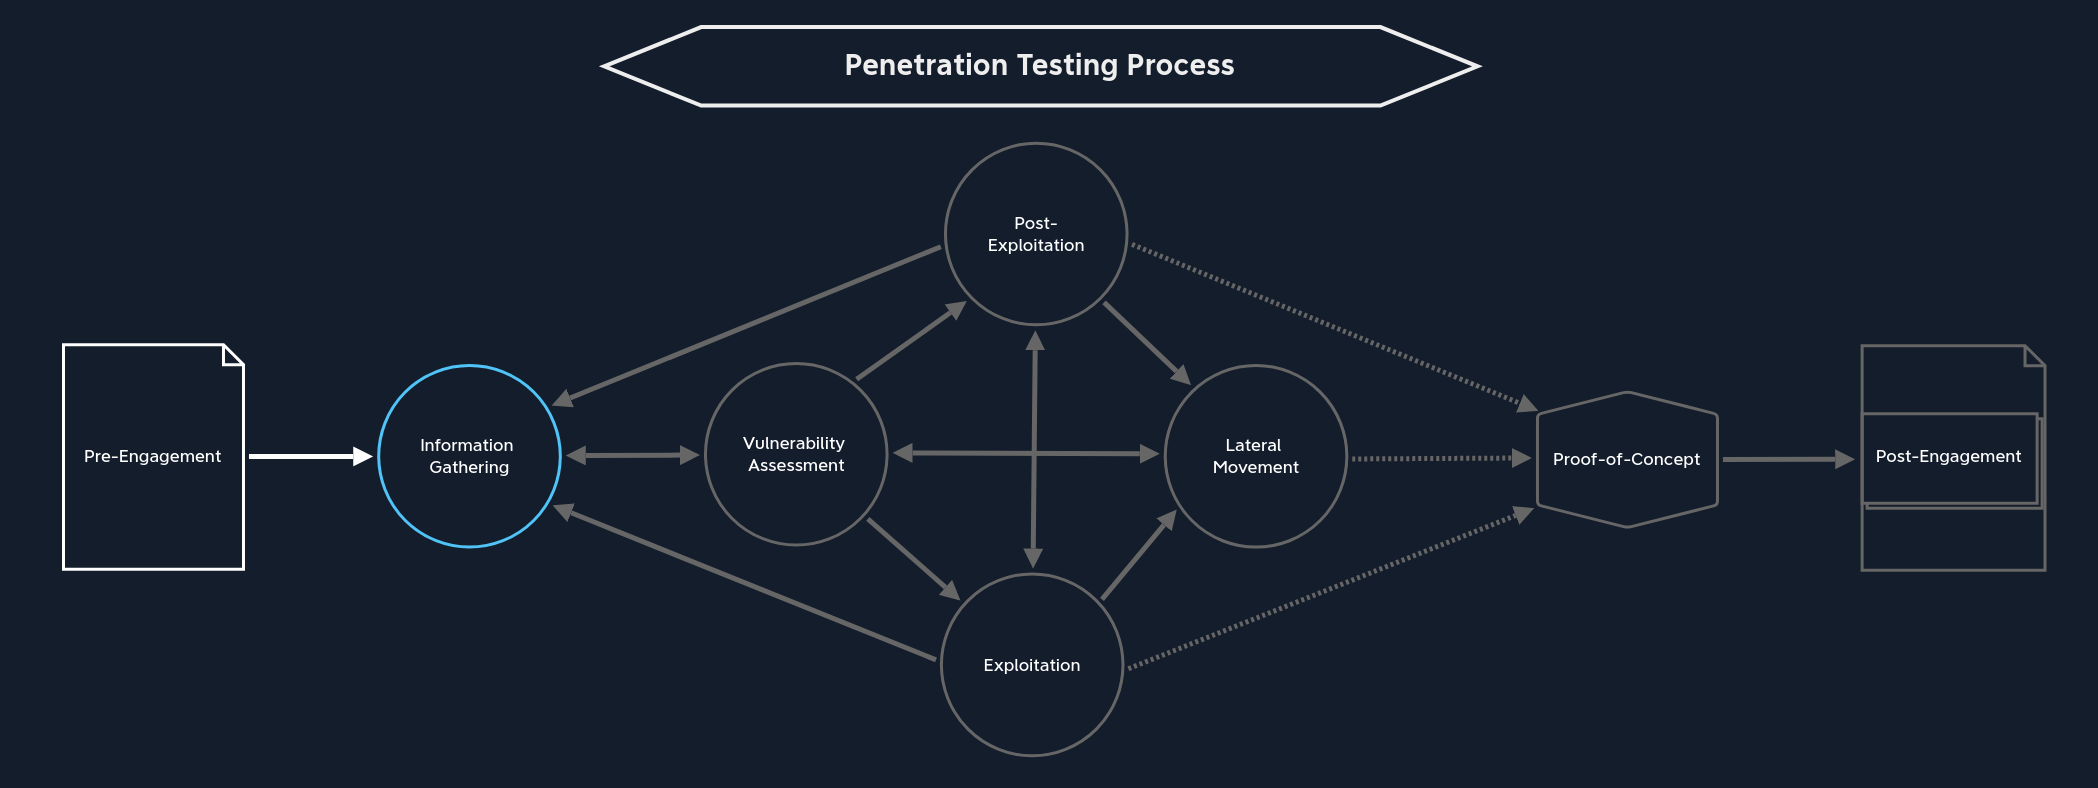
\includegraphics[width=\linewidth]{intro/process/images/pre.png}
  \caption{Pre-engagement}
  \label{fig:pentest-process-pre-engagement}
\end{figure}

The entire pre-engagement process consists of three essential components:
\begin{enumerate}
    \item Scoping questionnaire
    \item Pre-engagement meeting
    \item Kick-off meeting
\end{enumerate}

Before any of these can be discussed establish a NDA signed by all parties.
\begin{tabular}{ll}
Document &	Timing for Creation\\
Non-Disclosure Agreement (NDA) &	After Initial Contact \\
Scoping Questionnaire &	Before the Pre-Engagement Meeting \\
Scoping Document &	During the Pre-Engagement Meeting \\
Penetration Testing Proposal (Contract/Scope of Work (SoW)) &	During the
Pre-engagement Meeting\\
Rules of Engagement (RoE) &	Before the Kick-Off Meeting \\
Contractors Agreement (Physical Assessments) &	Before the Kick-Off Meeting \\
Reports &	During and after the conducted Penetration Test \\
\end{tabular}

\subsection{Scoping Questionnaire}

After initial contact is made with the client, we typically send them a Scoping Questionnaire to better understand the services they are seeking. This scoping questionnaire should clearly explain our services and may typically ask them to choose one or more from the following list:

\begin{tabular}{ll}
Internal Vulnerability Assessment &	 External Vulnerability Assessment\\
Internal Penetration Test &	 External Penetration Test\\
Wireless Security Assessment &	 Application Security Assessment\\
Physical Security Assessment &	 Social Engineering Assessment\\
Red Team Assessment &	 Web Application Security Assessment\\
\end{tabular}

nder each of these, the questionnaire should allow the client to be more
specific about the required assessment. Do they need a web application or
mobile application assessment? Secure code review? Should the Internal
Penetration Test be black box and semi-evasive? Do they want just a Phishing
assessment as part of the Social Engineering Assessment or also Vishing calls?
This is our chance to explain the depth and breadth of our services, ensure
that we understand our client's needs and expectations, and ensure that we can
adequately deliver the assessment they require.

Aside from the assessment type, client name, address, and key personnel contact information, some other critical pieces of information include:
\begin{itemize}
        \item How many expected live hosts?
        \item How many IPs/CIDR ranges in scope?
        \item How many Domains/Subdomains are in scope?
        \item How many wireless SSIDs in scope?
        \item How many web/mobile applications? If testing is authenticated, how many roles (standard user, admin, etc.)?
        \item For a Phishing assessment, how many users will be targeted? Will the client provide a list, or we will be required to gather this list via OSINT?
        \item If the client is requesting a Physical Assessment, how many locations? If multiple sites are in-scope, are they geographically dispersed?
        \item What is the objective of the Red Team Assessment? Are any activities (such as Phishing or physical security attacks) out of scope?
        \item Is a separate Active Directory Security Assessment desired?
        \item Will network testing be conducted from an anonymous user on the network or a standard domain user?
        \item Do we need to bypass Network Access Control (NAC)?
\end{itemize}

Finally, we will want to ask about information disclosure and evasiveness (if applicable to the assessment type):

\begin{itemize}
        \item Is the Penetration Test black box (no information provided), grey box (only IP address/CIDR ranges/URLs provided), white box (detailed information provided)

        \item Would they like us to test from a non-evasive, hybrid-evasive (start quiet and gradually become "louder" to assess at what level the client's security personnel detect our activities), or fully evasive.
\end{itemize}


\subsection{Pre-Engagement Meeting}
This meeting discusses all relevant and essential components with the customer before the penetration test, explaining them to our customer. The information we gather during this phase, along with the data collected from the scoping questionnaire, will serve as inputs to the Penetration Testing Proposal, also known as the Contract or Scope of Work (SoW).
\subsubsection{Contract checklist}
\begin{itemize}
\item {\emph NDA}
\item  Goals 	Goals are milestones that must be achieved during the order/project. In this process, goal setting is started with the significant goals and continued with fine-grained and small ones.
\item  {\emph Scope} 	The individual components to be tested are discussed and defined. These may include domains, IP ranges, individual hosts, specific accounts, security systems, etc. Our customers may expect us to find out one or the other point by ourselves. However, the legal basis for testing the individual components has the highest priority here.
\item  {\emph Penetration Testing Type} 	When choosing the type of penetration test, we present the individual options and explain the advantages and disadvantages. Since we already know the goals and scope of our customers, we can and should also make a recommendation on what we advise and justify our recommendation accordingly. Which type is used in the end is the client's decision.
\item  {\emph Methodologies} 	Examples: OSSTMM, OWASP, automated and manual unauthenticated analysis of the internal and external network components, vulnerability assessments of network components and web applications, vulnerability threat vectorization, verification and exploitation, and exploit development to facilitate evasion techniques.
\item  {\emph Penetration Testing Locations} 	External: Remote (via secure VPN) and/or Internal: Internal or Remote (via secure VPN)
\item  {\emph Time Estimation} 	For the time estimation, we need the start and the end date for the penetration test. This gives us a precise time window to perform the test and helps us plan our procedure. It is also vital to explicitly ask how time windows the individual attacks (Exploitation / Post-Exploitation / Lateral Movement) are to be carried out. These can be carried out during or outside regular working hours. When testing outside regular working hours, the focus is more on the security solutions and systems that should withstand our attacks.
\item  {\emph Third Parties} 	For the third parties, it must be determined via which third-party providers our customer obtains services. These can be cloud providers, ISPs, and other hosting providers. Our client must obtain written consent from these providers describing that they agree and are aware that certain parts of their service will be subject to a simulated hacking attack. It is also highly advisable to require the contractor to forward the third-party permission sent to us so that we have actual confirmation that this permission has indeed been obtained.
\item  {\emph Evasive Testing} 	Evasive testing is the test of evading and passing security traffic and security systems in the customer's infrastructure. We look for techniques that allow us to find out information about the internal components and attack them. It depends on whether our contractor wants us to use such techniques or not.
\item  {\emph Risks} 	We must also inform our client about the risks involved in the tests and the possible consequences. Based on the risks and their potential severity, we can then set the limitations together and take certain precautions.
\item  {\emph Scope Limitations  \& Restrictions} 	It is also essential to determine which servers, workstations, or other network components are essential for the client's proper functioning and its customers. We will have to avoid these and must not influence them any further, as this could lead to critical technical errors that could also affect our client's customers in production.
\item  {\emph Information Handling} 	HIPAA, PCI, HITRUST, FISMA/NIST, etc.
\item  {\emph Contact Information} 	For the contact information, we need to create a list of each person's name, title, job title, e-mail address, phone number, office phone number, and an escalation priority order.
\item  {\emph Lines of Communication} 	It should also be documented which communication channels are used to exchange information between the customer and us. This may involve e-mail correspondence, telephone calls, or personal meetings.
\item  {\emph Reporting} 	Apart from the report's structure, any customer-specific requirements the report should contain are also discussed. In addition, we clarify how the reporting is to take place and whether a presentation of the results is desired.
\item  {\emph Payment Terms} 	Finally, prices and the terms of payment are explained.
\end{itemize}

The most crucial element of this meeting is the detailed presentation of the
penetration test to our client and its focus. As we already know, each piece of
infrastructure is unique for the most part, and each client has particular
preferences on which they place the most importance. Finding out these
priorities is an essential part of this meeting.
\subsubsection{Rules of Engagement - Checklist}
\begin{itemize}
    \item {\emph Introduction} 	Description of this document.
    \item {\emph Contractor} 	Company name, contractor full name, job title.
    \item {\emph Penetration Testers} 	Company name, pentesters full name.
    \item {\emph Contact Information} 	Mailing addresses, e-mail addresses, and phone numbers of all client parties and penetration testers.
    \item {\emph Purpose} 	Description of the purpose for the conducted penetration test.
    \item {\emph Goals} 	Description of the goals that should be achieved with the penetration test.
    \item {\emph Scope} 	All IPs, domain names, URLs, or CIDR ranges.
    \item {\emph Lines of Communication} 	Online conferences or phone calls or face-to-face meetings, or via e-mail.
    \item {\emph Time Estimation} 	Start and end dates.
    \item {\emph Time of the Day to Test} 	Times of the day to test.
    \item {\emph Penetration Testing Type} 	External/Internal Penetration Test/Vulnerability Assessments/Social Engineering.
    \item {\emph Penetration Testing Locations} 	Description of how the connection to the client network is established.
    \item {\emph Methodologies} 	OSSTMM, PTES, OWASP, and others.
    \item {\emph Objectives / Flags} 	Users, specific files, specific information, and others.
    \item {\emph Evidence Handling} 	Encryption, secure protocols
    \item {\emph System Backups} 	Configuration files, databases, and others.
    \item {\emph Information Handling} 	Strong data encryption
    \item {\emph Incident Handling and Reporting} 	Cases for contact, pentest interruptions, type of reports
    \item {\emph Status Meetings} 	Frequency of meetings, dates, times, included parties
    \item {\emph Reporting} 	Type, target readers, focus
    \item {\emph Retesting} 	Start and end dates
    \item {\emph Disclaimers and Limitation of Liability} 	System damage, data loss
    \item {\emph Permission to Test} 	Signed contract, contractors agreement
\end{itemize}

\subsection{Kick-Off Meeting}

 We will go over the nature of the penetration test and how it will take place.
 Usually, there is no Denial of Service (DoS) testing. We also explain that if
 a critical vulnerability is identified, penetration testing activities will be
 paused, a vulnerability notification report will be generated, and the
 emergency contacts will be contacted. Typically these are only generated
 during External Penetration Tests for critical flaws such as unauthenticated
 remote code execution (RCE), SQL injection, or another flaw that leads to
 sensitive data disclosure. The purpose of this notification is to allow the
 client to assess the risk internally and determine if the issue warrants an
 emergency fix. We would typically only stop an Internal Penetration Test and
 alert the client if a system becomes unresponsive, we find evidence of illegal
 activity (such as illegal content on a file share) or the presence of an
 external threat actor in the network or a prior breach.

 xplaining the penetration testing process gives everyone involved a clear idea of our entire process. This demonstrates our professional approach and convinces our questioners that we know what we are doing. Because apart from the technical staff, CTO, and CISO, it will sound like a certain kind of magic that is very difficult for non-technical professionals to understand. So we must be mindful of our audience and target the most technically inexperienced questioner so our approach can be followed by everyone we talk to.

All points related to testing need to be discussed and clarified. It is crucial to respond precisely to the wishes and expectations of the customer/client. Every company structure and network is different and requires an adapted approach. Each client has different goals, and we should adjust our testing to their wishes. We can typically see how experienced our clients are in undergoing penetration tests early in the call, so we may have to shift our focus to explain things in more detail and be prepared to field more questions, or the kickoff call may be very quick and straightforward.

\subsection{Contractors Agreement}
f the penetration test also includes physical testing, then an additional
contractor's agreement is required. Since it is not only a virtual environment
but also a physical intrusion, completely different laws apply here. It is also
possible that many of the employees have not been informed about the test.
Suppose we encounter employees with a very high-security awareness during the
physical attack and social engineering attempts, and we get caught. In that
case, the employees will, in most cases, contact the police. This additional
contractor's agreement is our "get out of jail free card" in this case. 

Checkpoint:
\begin{itemize}
\item Introduction
\item Contractor
\item Purpose
\item Goal
\item Penetration Testers
\item Contact Information
\item Physical Addresses
\item Building Name
\item Floors
\item Physical Room Identifications
\item Physical Components
\item Timeline
\item Notarization
\item Permission to Test
\end{itemize}

\input{intro/process/Int}
\section{Vulnerability Assessment}

During the vulnerability assessment phase, we examine and analyze the information gathered during the information gathering phase. The vulnerability assessment phase is an analytical process based on the findings.

\begin{figure}
  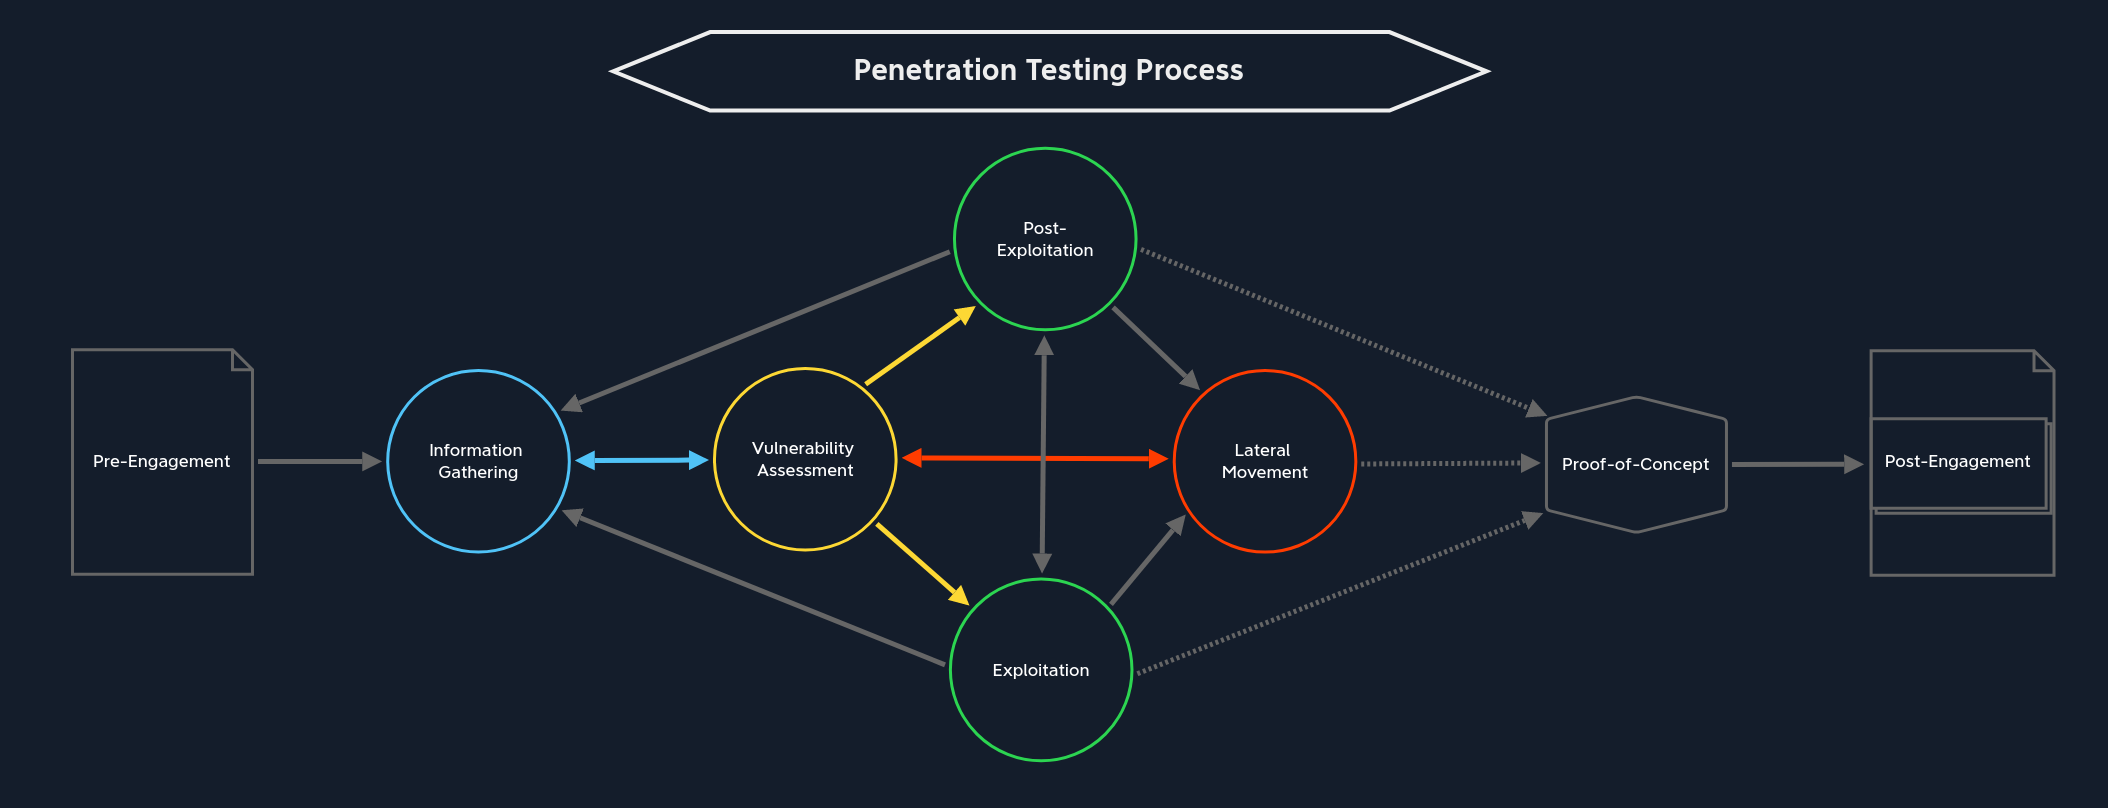
\includegraphics[width=\linewidth]{intro/process/images/vuln.png}
  \caption{Vulnerability Assessment}
  \label{fig:pentest-process-vuln-assessment}
\end{figure}

An analysis is a detailed examination of an event or process, describing its
origin and impact, that with the help of certain precautions and actions, can
be triggered to support or prevent future occurrences.

here are four different types of analysis:
\begin{itemize}
    \item {\bf Descriptive} essential in any data analysis. On the one hand, it describes a data set based on individual characteristics. It helps to detect possible errors in data collection or outliers in the data set.
    \item {\bf Diagnostic} clarifies conditions' causes, effects, and interactions. Doing so provides insights that are obtained through correlations and interpretation. We must take a backward-looking view, similar to descriptive analysis, with the subtle difference that we try to find reasons for events and developments.
    \item {\bf Predictive} 	By evaluating historical and current data, predictive analysis creates a predictive model for future probabilities. Based on the results of descriptive and diagnostic analyses, this method of data analysis makes it possible to identify trends, detect deviations from expected values at an early stage, and predict future occurrences as accurately as possible.
    \item {\bf Prescriptive} 	Prescriptive analytics aims to narrow down what actions to take to eliminate or prevent a future problem or trigger a specific activity or process.
\end{itemize}

\subsection{Vulnerability Research and Analysis}
Information Gathering and Vulnerability Research can be considered a part of
{\bf descriptive} analysis. In Vulnerability Research, we look for known
vulnerabilities, exploits, and security holes that have already been discovered
and reported. Therefore, if we have identified a version of a service or
application through information gathering and found a Common Vulnerabilities
and Exposures (CVE), it is very likely that this vulnerability is still
present.

This is where {\bf Diagnostic} analysis and {\bf Predictive} analysis is used. Once we have
found a published vulnerability like this, we can diagnose it to determine what
is causing or has caused the vulnerability. Here, we must understand the
functionality of the Proof-Of-Concept (POC) code or the application or service
itself as best as possible, as many manual configurations by administrators
will require some customization for the POC. Each POC is tailored to a specific
case that we will also need to adapt to ours in most cases.

\subsection{Assessment of Possible Attack Vectors}
Vulnerability Assessment also includes the actual testing, which is part of
{\bf Predictive} analysis. In doing so, we analyze historical information and
combine it with the current information that we have been able to find out.
Whether we have received specific evasion level requirements from our client,
we test the services and applications found locally or on the target system. If
we have to test covertly and avoid alerts, we should mirror the target system
locally as precisely as possible. This means we use the information obtained
during our information gathering phase to replicate the target system and then
look for vulnerabilities in the locally deployed system.

\subsection{The return}
Suppose we are unable to detect or identify potential vulnerabilities from our
analysis. In that case, we will return to the Information Gathering stage and
look for more in-depth information than we have gathered so far. It is
important to note that these two stages (Information Gathering and
Vulnerability Assessment) often overlap, resulting in regular back and forth
movement between them. We will see this in many videos where the author is
solving an HTB box or some CTF challenge. We should remember that these
challenges are often solved as fast as possible, and therefore speed is more
important than quality. In a CTF, the goal is to get on the target machine and
capture the flags with the highest privileges as fast as possible instead of
exposing all potential weaknesses in the system.

A (real) Penetration Test is not a CTF.

Here the quality and intensity of our penetration test and its analysis have
the highest priority because nothing is worse if our client gets successfully
hacked via a relatively simple vector that we should have uncovered during our
penetration test.




\section{Exploitation}

\begin{figure}
  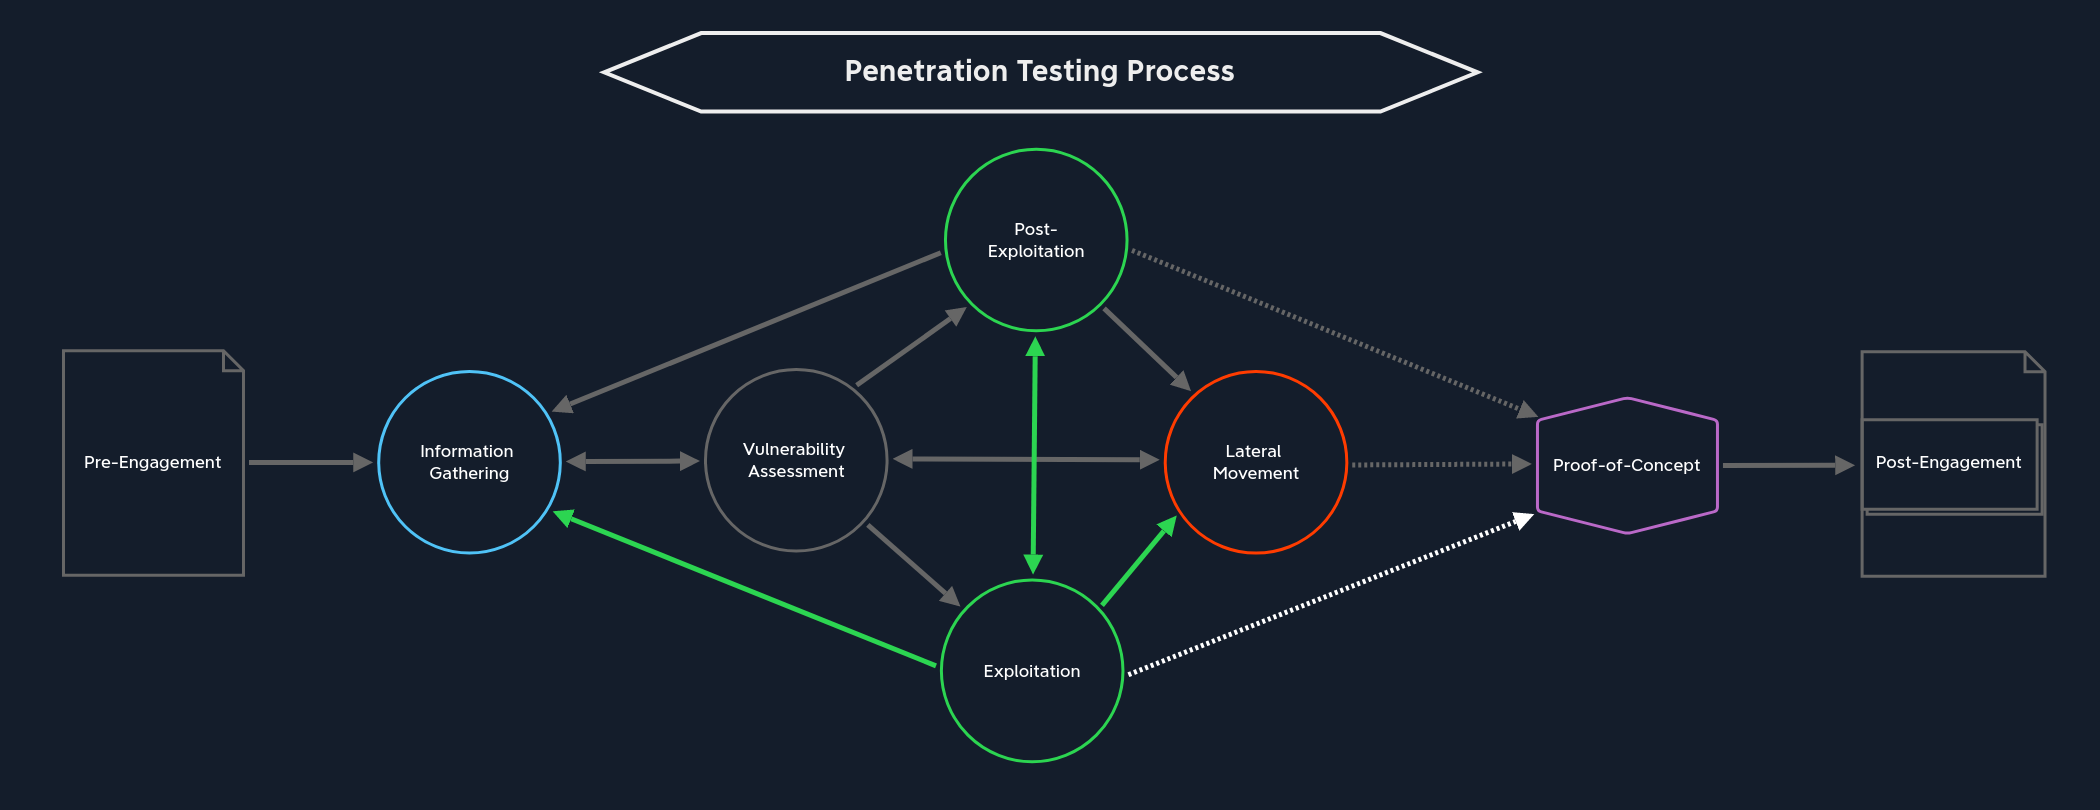
\includegraphics[width=\linewidth]{intro/process/images/exploit.png}
  \caption{Exploitation}
  \label{fig:pentest-process-exploit}
\end{figure}
During the Exploitation stage, we look for ways that these weaknesses can be
adapted to our use case to obtain the desired role (i.e., a foothold, escalated
privileges, etc.). If we want to get a reverse shell, we need to modify the PoC
to execute the code, so the target system connects back to us over (ideally) an
encrypted connection to an IP address we specify. Therefore, the preparation of
an exploit is mainly part of the Exploitation stage.

These stages should not be strictly separated from each other, as they are
closely connected. Nevertheless, it is still important to distinguish which
phase we are in and its purpose. Because later, with much more complex
processes and much more information, it is very easy to lose track of the steps
that have been taken, especially if the penetration test lasts several weeks
and covers a massive scope.

\subsection{Prioritization of Possible Attacks}
Once we have found one or two vulnerabilities during the Vulnerability
Assessment stage that we can apply to our target network/system, we can
prioritize those attacks. Which of those attacks we prioritize higher than the
others depends on the following factors:
\begin{itemize}
    \item  Probability of Success
    \item  Complexity
    \item  Probability of Damage
\end{itemize}

First, we need to assess the probability of successfully executing a particular
attack against the target. \href{https://nvd.nist.gov/vuln-metrics/cvss}{CVSS
Scoring} can help us here, using the
\href{https://nvd.nist.gov/vuln-metrics/cvss/v3-calculator}{NVD calculator}
better to calculate the specific attacks and their probability of success.

Complexity represents the effort of exploiting a specific vulnerability. This
is used to estimate how much time, effort, and research is required to execute
the attack on the system successfully. Our experience plays an important role
here because if we are to carry out an attack that we have never used before,
this will logically require much more research and effort since we must
understand the attack and the exploit structure in detail before applying it.

Estimating the probability of damage caused by the execution of an exploit
plays a critical role, as we must avoid any damage to the target systems.
Generally, we do not perform DoS attacks unless our client requires them.
Nevertheless, attacking the running services live with exploits that can cause
damage to the software or the operating system is something that we must avoid
at all times.


\subsection{Preparation for the Attack}
Sometimes we will run into a situation where we can't find high-quality, known
working PoC exploit code. Therefore, it may be necessary to reconstruct the
exploit locally on a VM representing our target host to figure out precisely
what needs to be adapted and changed. Once we have set up the system locally
and installed known components to mirror the target environment as closely as
possible (i.e., same version numbers for target services/applications), we can
start preparing the exploit by following the steps described in the exploit.
Then we test this on a locally hosted VM to ensure it works and does not damage
significantly. In other situations, we will encounter misconfigurations and
vulnerabilities that we see very often and know exactly which tool or exploit
to use and whether the exploit or technique is "safe" or can cause
instability.

If ever in doubt before running an attack, it's always best to check with our
client, providing them all necessary data so they can make an informed decision
on whether they would like us to attempt exploitation or just mark the finding
as an issue. If they opt for us not to proceed with exploitation, we can note
in the report that it was not confirmed actively but is likely an issue that
needs to be addressed. We have a certain amount of leeway during penetration
tests and should always use our best judgment if a particular attack seems too
risky or could potentially cause a disruption. When in doubt, communicate. Your
team lead/manager, the client, will almost certainly prefer extra communication
than run into a situation where they are trying to bring a system back online
after a failed exploit attempt.

Once we have successfully exploited a target and have initial access (and taken
clear notes for our reports and logged all activities in our activity log!),
we'll move on to the post-exploitation and lateral movement stages.

\section{Post-Exploitation}

\begin{figure}
  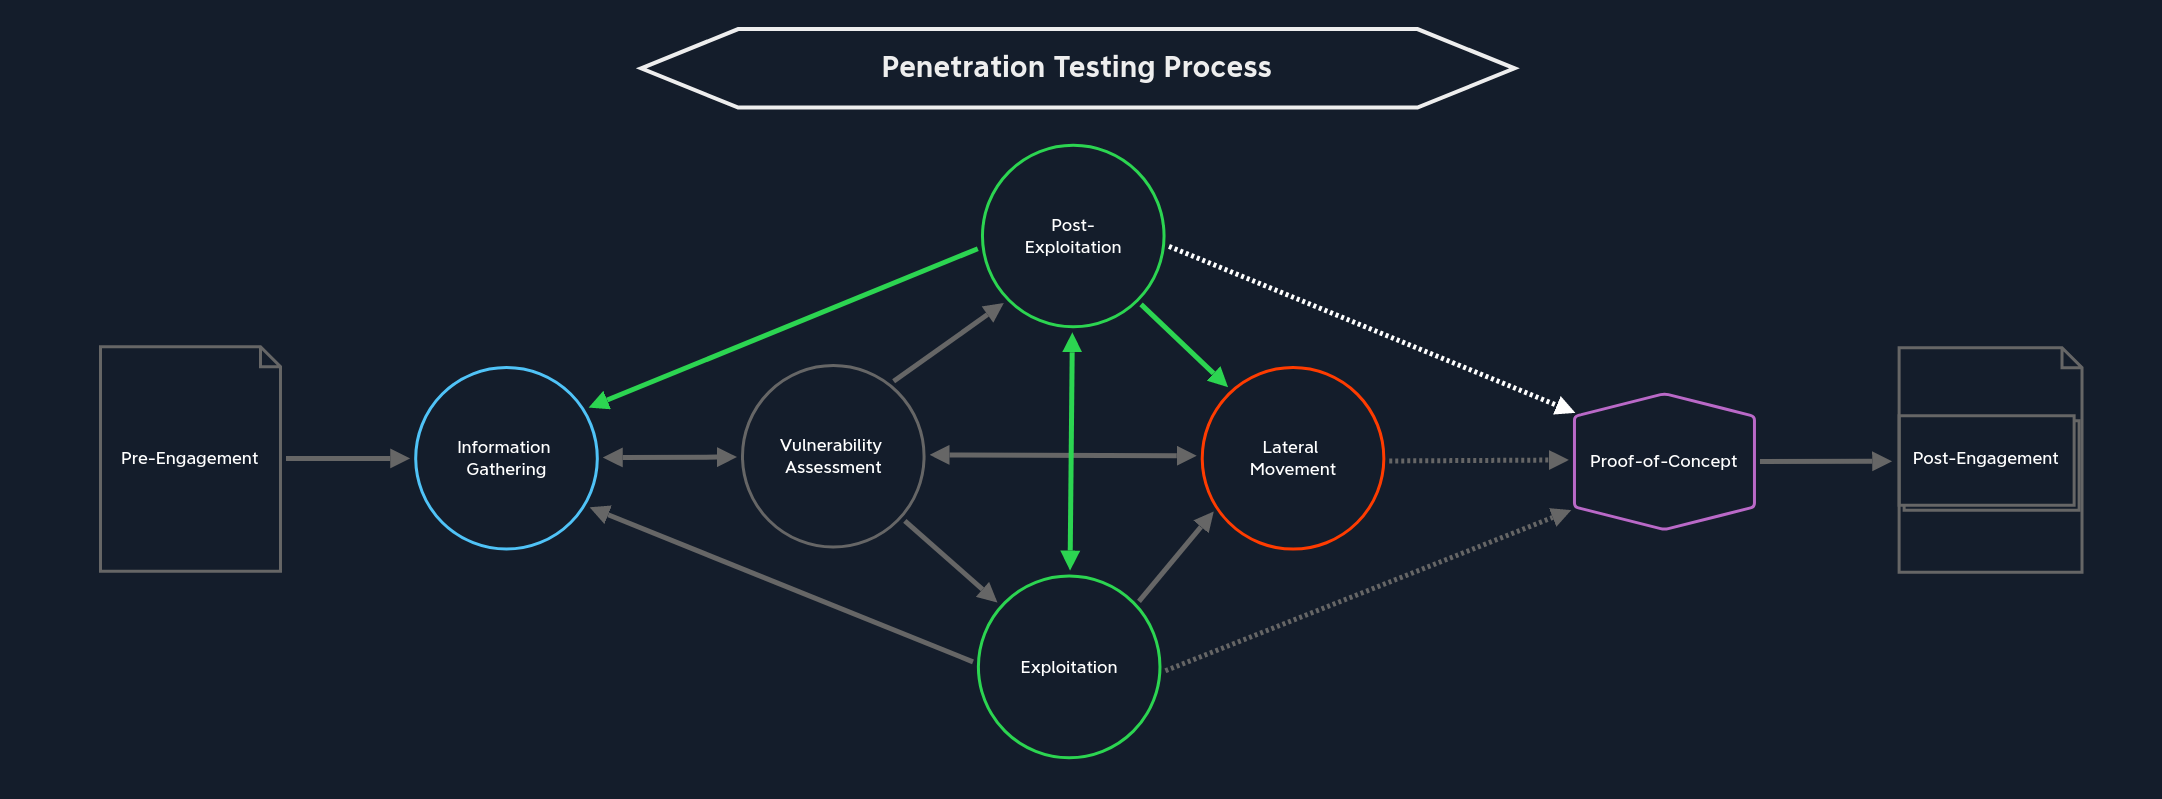
\includegraphics[width=\linewidth]{intro/process/images/post.png}
  \caption{Post-Exploitation}
  \label{fig:pentest-process-post-exploit}
\end{figure}

 The Post-Exploitation stage aims to obtain sensitive and security-relevant
 information from a local perspective and business-relevant information that,
 in most cases, requires higher privileges than a standard user. This stage
 includes the following components:

 \begin{tabular}{ll}
 Evasive Testing &	Information Gathering \\
Pillaging &	Vulnerability Assessment \\
Privilege Escalation &	Persistence \\
Data Exfiltration & \\
\end{tabular}

\subsection{Evasive Testing}
If a skilled administrator monitors the systems, any change or even a single
command could trigger an alarm that will give us away. In many cases, we get
kicked out of the network, and then threat hunting begins where we are the
focus. We may also lose access to a host (that gets quarantined) or a user
account (that gets temporarily disabled or the password changed). This
penetration test would have failed but succeeded in some ways because the
client could detect some actions. We can provide value to the client in this
situation by still writing up an entire attack chain and helping them identify
gaps in their monitoring and processes where they did not notice our actions.
For us, we can study how and why the client detected us and work on improving
our evasion skills. Perhaps we did not thoroughly test a payload, or we got
careless and ran a command such as \verb+net user+ or \verb+whoami+ that is
often monitored by EDR systems and flagged as anomalous activity. 

Evasive testing is divided into three different categories:
Evasive, Hybrid Evasive and Non-Evasive

This does not mean that we cannot use all three methods. Suppose our client
wants to perform an intrusive penetration test to get as much information as
possible and the most in-depth testing results. In that case, we will perform
Non-Evasive Testing, as the security measures around the network may limit and
even stop us. However, this can also be combined with Evasive testing, using
the same commands and methods for non-evasive testing. We can then see if the
security measures can identify and respond to the actions performed. In
Hybrid-Evasive testing, we can test specific components and security measures
that have been defined in advance. This is common when the customer only wants
to test specific departments or servers to see if they can withstand the
attacks.

\subsection{Information Gathering}

Since we have gained a new perspective on the system and the network of our
target system in the Exploitation stage, we are basically in a new environment.
This means we first have to reacquaint ourselves with what we are working with
and what options are available. Therefore, in the Post-Exploitation stage, we
go through the Information Gathering and Vulnerability Assessment stages again,
which we can consider as parts of the current stage. This is because the
information we had up to this point was gathered from an external perspective,
not an internal one.

From the inside (local) perspective, we have many more possibilities and
alternatives to access certain information that is relevant to us. Therefore,
the information gathering stage starts all over again from the local
perspective. We search and gather as much information as we can. The difference
here is that we also enumerate the local network and local services such as
printers, database servers, virtualization services, etc. Often we will find
shares intended for employees to use to exchange and share data and files. The
investigation of these services and network components is called Pillaging.

\subsection{Pillaging}

Pillaging is the stage where we examine the role of the host in the corporate
network. We analyze the network configurations, including but not limited to:
Interfaces, Routing, DNS, ARP\ldots

Understanding the role of the system we are on also gives us an excellent
understanding of how it communicates with other network devices and its
purpose. From this, we can find out, for example, what alternative subdomains
exist, whether it has multiple network interfaces, whether there are other
hosts with which this system communicates, if admins are connecting to other
hosts from it, and if we can potentially reuse credentials or steal an SSH key
to further our access or establish persistence, etc. This helps, above all, to
get an overview of the network's structure.

During the pillaging stage, we will also hunt for sensitive data such as
passwords on shares, local machines, in scripts, configuration files, password
vaults, documents (Excel, Word, .txt files, etc.), and even email.

Our main goals with pillaging are to show the impact of successful exploitation
and, if we have not yet reached the goal of the assessment, to find additional
data such as passwords that can be inputs to other stages such as lateral
movement. 


\subsection{Persistence}

Once we have an overview of the system, our immediate next step is maintaining
access to the exploited host. This way, if the connection is interrupted, we
can still access it. This step is essential and often used as the first step
before the Information Gathering and Pillaging stages.

We should follow non-standardized sequences because each system is individually
configured by a unique administrator who brings their own preferences and
knowledge. It is recommended that we work flexibly during this phase and adapt
to the circumstances. For example, suppose we have used a buffer overflow
attack on a service that is likely to crash it. In that case, we should
establish persistence to the system as soon as possible to avoid having to
attack the service multiple times and potentially causing a disruption. Often
if we lose the connection, we will not be able to access the system in the same
way.

\subsection{Vulnerability Assessment}

If we can maintain access and have a good overview of the system, we can use
the information about the system and its services and any other data stored on
it to repeat the Vulnerability Assessment stage, but this time from inside the
system. We analyze the information and prioritize it accordingly. The goal we
pursue next is the escalation of privileges (if not already in place).

Again, it is essential to distinguish between exploits that can harm the system
and attacks against the services that do not cause any disruption. In doing so,
we weigh the components we have already gone through in the first Vulnerability
Assessment stage.

\subsection{Privilege Escalation}

Privilege escalation is significant, and in most cases, it represents a
critical moment that can open many more new doors for us. Getting the highest
possible privileges on the system or domain is often crucial. Therefore we want
to get the privileges of the root (on Linux-based systems) or the domain
administrator/local administrator/SYSTEM (on Windows-based systems) because
this will often allow us to move through the entire network without any
restrictions.

However, it is essential to remember that the escalation of privileges does not
always have to occur locally on the system. We can also obtain stored
credentials during the information gathering stage from other users who are
members of a higher privileged group. Exploiting these privileges to log in as
another user is also part of privilege escalation because we have escalated our
privileges (quickly) using the new set of credentials.

\subsection{Data Exfiltration}

During the Information Gathering and Pillaging stage, we will often be able to
find, among other things, considerable personal information and customer data.
Some clients will want to check whether it is possible to exfiltrate these
types of data. Security systems such as Data Loss Prevention (DLP) and
Endpoint Detection and Response (EDR) help detect and prevent data
exfiltration. In addition to Network Monitoring, many companies use encryption
on hard drives to prevent external parties from viewing such information.
Before exfiltrating any actual data, we should check with the customer and our
manager. It can often be enough to create some bogus data (such as fake credit
card numbers or social security numbers) and exfiltrate it to our system. That
way, the protection mechanisms that look for patterns in data leaving the
network will be tested, but we will not be responsible for any live sensitive
data on our testing machine.

Companies must adhere to data security regulations depending on the type of
data involved. These include, but are not limited to:
Credit Card Account Information (Payment Card Industry (PCI)), Electronic
Patient Health Information 'Health Insurance Portability and Accountability Act
(HIPAA)), Consumers Private Banking Information (Gramm-Leach-Bliley (GLBA))
Government Information 	(Federal Information Security Management Act of 2002
(FISMA))

It is worth familiarizing ourselves with each of these frameworks but what is
crucial for us, however, is how we handle this information. For us, the type of
data does not have much significance, but the required controls around it do,
and as stated previously, we can simulate exfiltrating data from the network as
a proof of concept that it is possible. We should check with the client to
ensure that their systems are intended to catch the fake data type that we
attempt to exfiltrate if we are successful, so we do not misrepresent anything
in our report.

It's a good habit to run a screen recording (along with taking screenshots) as
additional evidence for such vital steps. If we only have terminal access, we
can display the hostname, IP address, user name, and the corresponding path to
the customer file and take a screenshot or screen capture. This helps us prove
where the data originated from and that we could remove it from the environment
successfully.

If sensitive data like this is found, our client should, of course, be informed
immediately. Based on the fact that we could escalate the privileges and
exfiltrate personal data, they may want to pause, end, or shift the focus of
the penetration test, especially if data exfiltration was the primary goal.
However, this is at our client's discretion, and many will prefer that we keep
testing to identify all possible weaknesses in their environment.


\section{Lateral movement}

\begin{figure}
  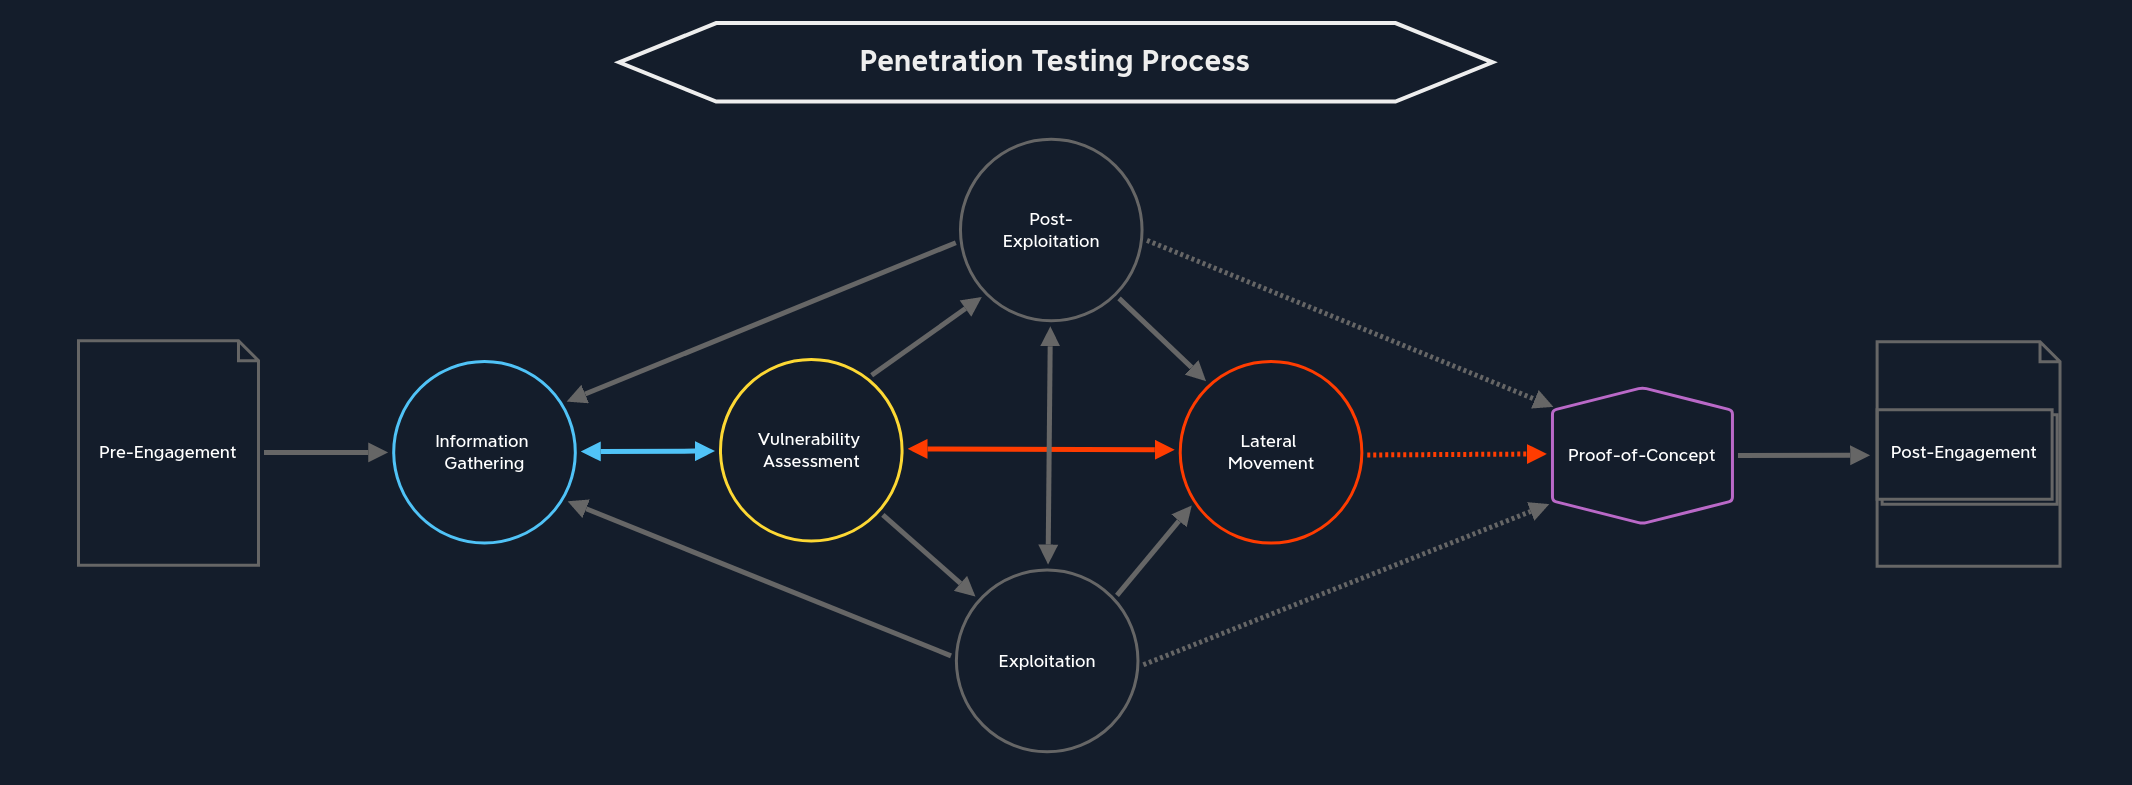
\includegraphics[width=\linewidth]{intro/process/images/lateral.png}
  \caption{Lateral movement}
  \label{fig:pentest-process-lateral}
\end{figure}

The goal here is that we test what an attacker could do within the entire
network. After all, the main goal is not only to successfully exploit a
publicly available system but also to get sensitive data or find all ways that
an attacker could render the network unusable. One of the most common examples
is ransomware. If a system in the corporate network is infected with
ransomware, it can spread across the entire network. It locks down all the
systems using various encryption methods, making them unusable for the whole
company until a decryption key is entered.

In the most common cases, the company is financially extorted to make a profit.
Often, it is only at this moment that companies realize how important IT
security is. If they had had a good penetration tester who had tested things
(and proper processes and layered defenses in place), they probably could have
prevented such a situation and the financial (if not legal) damage. It is often
forgotten that in many countries, the CEOs are held liable for not securing
their customer data appropriately.

In this stage, we want to test how far we can move manually in the entire network and what vulnerabilities we can find from the internal perspective that might be exploited. In doing so, we will again run through several phases:
\begin{itemize}
    \item  Pivoting
    \item  Evasive Testing
    \item  Information Gathering
    \item  Vulnerability Assessment
    \item  (Privilege) Exploitation
    \item  Post-Exploitation
\end{itemize}

As seen in the graphic above, we can move to this stage from the Exploitation and the Post-Exploitation stage. Sometimes we may not find a direct way to escalate our privileges on the target system itself, but we have ways to move around the network. This is where Lateral Movement comes into play.

\subsection{Pivoting}

In most cases, the system we use will not have the tools to enumerate the internal network efficiently. Some techniques allow us to use the exploited host as a proxy and perform all the scans from our attack machine or VM. In doing so, the exploited system represents and routes all our network requests sent from our attack machine to the internal network and its network components.

In this way, we make non-routable networks (and therefore publicly unreachable) can still be reached. This allows us to scan them for vulnerabilities and penetrate deeper into the network. This process is also known as Pivoting or Tunneling.

An elementary example could be that we have a printer at home that is not accessible from the Internet, but we can send print jobs from our home network. If one of the hosts on our home network has been compromised, it could be leveraged to send these jobs to the printer. Though this is a simple (an unlikely) example, it illustrates the goal of pivoting, which is to access inaccessible systems via an intermediary system.

\subsection{Evasive Testing}

Also, at this stage, we should consider whether evasive testing is part of the assessment scope. There are different procedures for each tactic, which support us in disguising these requests to not trigger an internal alarm among the administrators and the blue team.

There are many ways to protect against lateral movement, including network (micro) segmentation, threat monitoring, IPS/IDS, EDR, etc. To bypass these efficiently, we need to understand how they work and what they respond to. Then we can adapt and apply methods and strategies that help avoid detection.

\subsection{Information Gathering}

Before we target the internal network, we must first get an overview of which systems and how many can be reached from our system. This information may already be available to us from the last post-exploitation stage, where we took a closer look at the settings and configurations of the system.

We return to the Information Gathering stage, but this time, we do it from inside the network with a different view of it. Once we have discovered all hosts and servers, we can enumerate them individually.

\subsection{Vulnerability Assessment}

Vulnerability assessment from the inside of the network differs from the previous procedures. This is because far more errors occur inside a network than on hosts and servers exposed to the Internet. Here, the groups to which one has been assigned and the rights to different system components play an essential role. In addition, it is common for users to share information and documents and work on them together.

This type of information is of particular interest to us when planning our attacks. For example, if we compromise a user account assigned to a developer group, we may gain access to most of the resources used by company developers. This will likely provide us with crucial internal information about the systems and could help us to identify flaws or further our access.

\subsection{(Privilege) Exploitation}

Once we have found and prioritized these paths, we can jump to the step where we use these to access the other systems. We often find ways to crack passwords and hashes and gain higher privileges. Another standard method is to use our existing credentials on other systems. There will also be situations where we do not even have to crack the hashes but can use them directly. For example, we can use the tool Responder to intercept NTLMv2 hashes. If we can intercept a hash from an administrator, then we can use the pass-the-hash technique to log in as that administrator (in most cases) on multiple hosts and servers.

After all, the Lateral Movement stage aims to move through the internal network. Existing data and information can be versatile and often used in many ways.

\subsection{Post-Exploitation}

Once we have reached one or more hosts or servers, we go through the steps of the post-exploitation stage again for each system. Here we again collect system information, data from created users, and business information that can be presented as evidence. However, we must again consider how this different information must be handled and the rules defined around sensitive data in the contract.

\section{Proof of concept}

\begin{figure}
  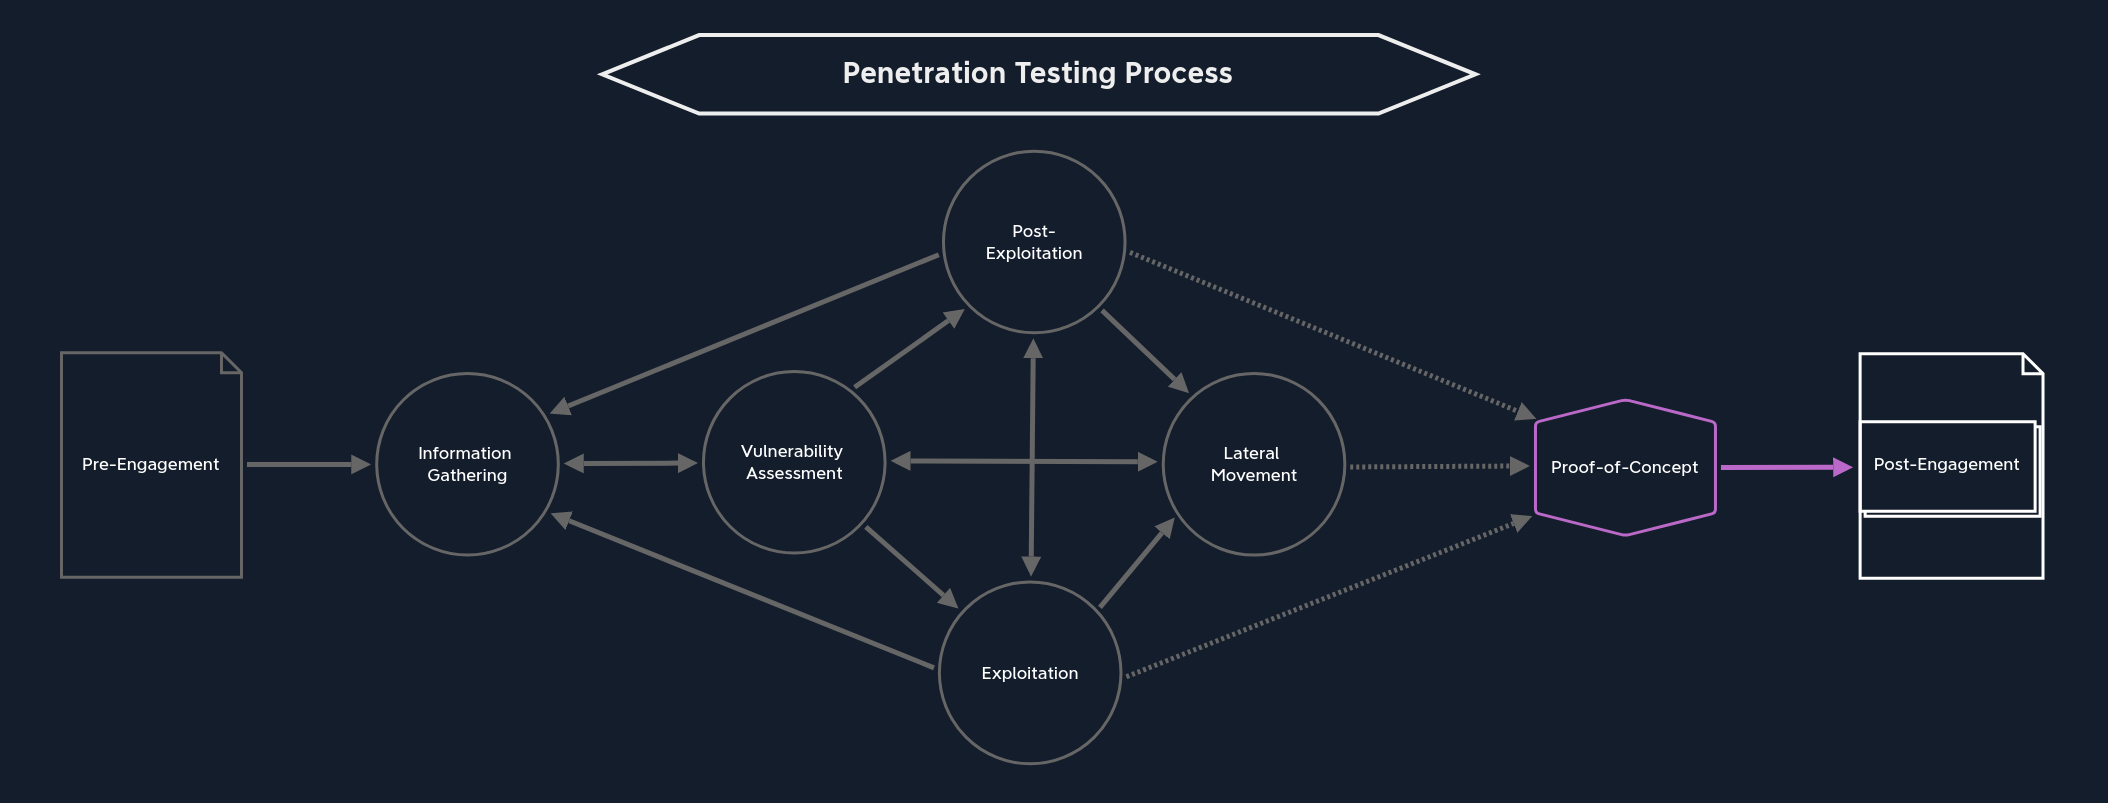
\includegraphics[width=\linewidth]{intro/process/images/poc.png}
  \caption{Proof of concept}
  \label{fig:pentest-process-poc}
\end{figure}

Proof of Concept (PoC) or Proof of Principle is a project management term. In
project management, it serves as proof that a project is feasible in principle.
The criteria for this can lie in technical or business factors. Therefore, it
is the basis for further work, in our case, the necessary steps to secure the
corporate network by confirming the discovered vulnerabilities. In other words,
it serves as a decision-making basis for the further course of action. At the
same time, it enables risks to be identified and minimized.

This project step is often integrated into the development process for new
application software (prototyping) or IT security solutions. For us in
information security, this is where we prove vulnerabilities in operating
systems or application software. We use this PoC to prove that a security
problem exists so that the developers or administrators can validate it,
reproduce it, see the impact, and test their remediation efforts. One of the
most common examples used to prove software vulnerabilities is executing the
calculator (calc.exe on Windows) on the target system. In principle, the PoC
also assesses the probability of success of system access from actual
exploitation.

A PoC can have many different representations. For example, documentation of
the vulnerabilities found can also constitute a PoC. The more practical version
of a PoC is a script or code that automatically exploits the vulnerabilities
found. This demonstrates the flawless exploitation of the vulnerabilities. This
variant is straightforward for an administrator or developer because they can
see what steps our script takes to exploit the vulnerability.

However, there is one significant disadvantage that has occurred from time to
time. Once the administrators and developers have received such a script from
us, it is easy for them to "fight" against our script. They focus on changing
the systems so that the script we created no longer works. The important thing
is that the script is only one way of exploiting a given vulnerability.
Therefore, working against our script instead of with it and modifying and
securing the systems so that our script no longer works does not mean that the
information obtained from the script cannot be obtained in another way. It is
an important aspect that should be discussed with the administrators and
developers and explicitly mentioned and pointed out.

The report they receive from us should help them see the entire picture, focus
on the broader issues, and provide clear remediation advice. Including an
attack chain walkthrough in the event of domain compromise during an internal
is a great way to show how multiple flaws can be combined and how fixing one
flaw will break the chain, but the other flaws will still exist. If these are
not also fixed, there may be another path to get to the point where the attack
chain was remediated and continue onwards. We should also drive this point home
during our report review meeting.

For example, if a user uses the password Password123, the underlying
vulnerability is not the password but the password policy. If a Domain Admin is
found to be using that password and it is changed, that one account will now
have a stronger password, but the problem of weak passwords will likely still
be endemic within the organization.

If the password policy followed high standards, the user would not be able to
use such a weak password. Administrators and developers are responsible for the
functionality and the quality of their systems and applications. Furthermore,
high quality stands for high standards, which we should emphasize through our
remediation recommendations.

\section{Post-Engagement}

\begin{figure}
  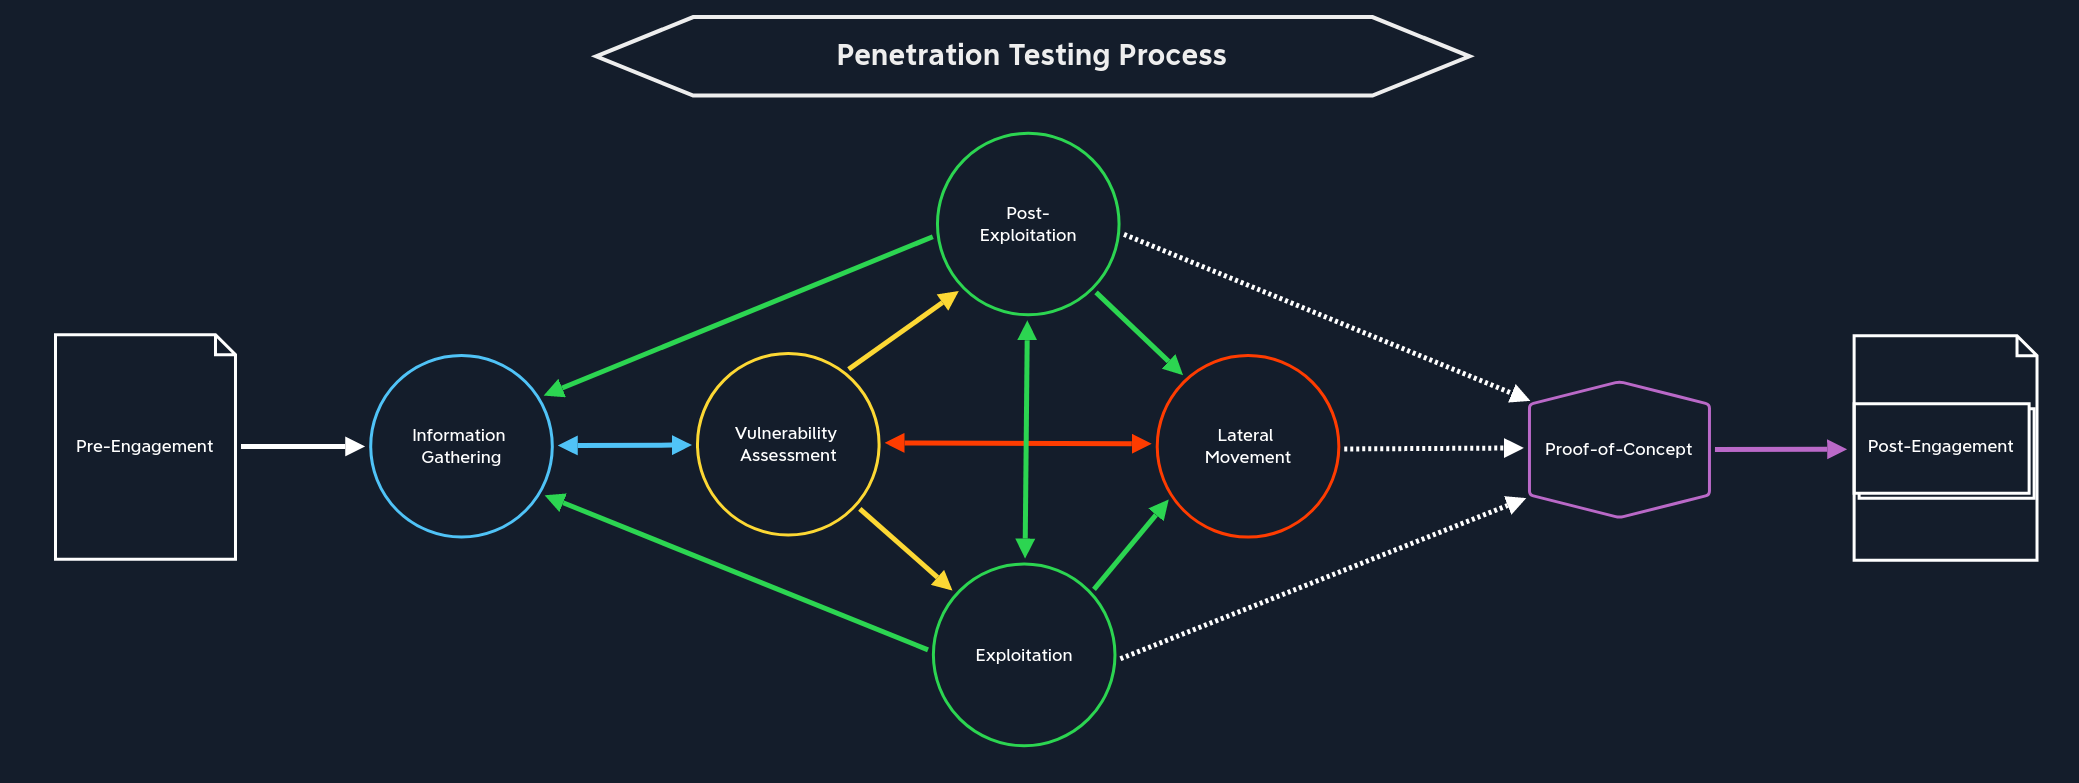
\includegraphics[width=\linewidth]{intro/process/images/post-engagement.png}
  \caption{Post-engagement}
  \label{fig:pentest-process-post-engagement}
\end{figure}

Much like there is considerable legwork before an engagement officially starts
(when testing begins), we must perform many activities (many of them
contractually binding) after our scans, exploitation, lateral movement, and
post-exploitation activities are complete. No two engagements are the same, so
these activities may differ slightly but generally must be performed to close
out an engagement fully.

\subsection{Cleanup}

Once testing is complete, we should perform any necessary cleanup, such as
deleting tools/scripts uploaded to target systems, reverting any (minor)
configuration changes we may have made, etc. We should have detailed notes of
all of our activities, making any cleanup activities easy and efficient. If we
cannot access a system where an artifact needs to be deleted, or another change
reverted, we should alert the client and list these issues in the report
appendices. Even if we can remove any uploaded files and revert changes (such
as adding a local admin account), we should document these changes in our
report appendices in case the client receives alerts that they need to follow
up on and confirm that the activity in question was part of our sanctioned
testing.

\subsection{Documentation and Reporting}

Before completing the assessment and disconnecting from the client's internal
network or sending "stop" notification emails to signal the end of testing
(meaning no more interaction with the client's hosts), we must make sure to
have adequate documentation for all findings that we plan to include in our
report. This includes command output, screenshots, a listing of affected hosts,
and anything else specific to the client environment or finding. We should also
make sure that we have retrieved all scan and log output if the client hosted a
VM in their infrastructure for an internal penetration test and any other data
that may be included as part of the report or as supplementary documentation.
We should not keep any Personal Identifiable Information (PII), potentially
incriminating info, or other sensitive data we came across throughout testing.

\subsection{Report Review Meeting}

Once the draft report is delivered, and the client has had a chance to
distribute it internally and review it in-depth, it is customary to hold a
report review meeting to walk through the assessment results. The report review
meeting typically includes the same folks from the client and the firm
performing the assessment. Depending on the types of findings, the client may
bring in additional technical subject matter experts if the finding is related
to a system or application they are responsible for. Typically we will not read
the entire report word for word but walk through each finding briefly and give
an explanation from our own perspective/experience. The client will have the
opportunity to ask questions about anything in the report, ask for
clarifications, or point out issues that need to be corrected. Often the client
will come with a list of questions about specific findings and will not want to
cover every finding in detail (such as low-risk ones).

\subsection{Deliverable Acceptance}

The Scope of Work should clearly define the acceptance of any project
deliverables. In penetration test assessments, generally, we deliver a report
marked DRAFT and give the client a chance to review and comment. Once the
client has submitted feedback (i.e., management responses, requests for
clarification/changes, additional evidence, etc.) either by email or (ideally)
during a report review meeting, we can issue them a new version of the report
marked FINAL. Some audit firms that clients may be beholden to will not accept
a penetration test report with a DRAFT designation. Other companies will not
care, but keeping a uniform approach across all customers is best.

\subsection{Post-Remediation Testing}

Most engagements include post-remediation testing as part of the project's
total cost. In this phase, we will review any documentation provided by the
client showing evidence of remediation or just a list of remediated findings.
We will need to reaccess the target environment and test each issue to ensure
it was appropriately remediated. We will issue a post-remediation report that
clearly shows the state of the environment before and after post-remediation
testing.

\subsection{Data Retention}

After a penetration test concludes, we will have a considerable amount of
client-specific data such as scan results, log output, credentials,
screenshots, and more. Data retention and destruction requirements may differ
from country to country and firm to firm, and procedures surrounding each
should be outlined clearly in the contract language of the Scope of Work and
the Rules of Engagement.

We should retain evidence for some time after the penetration test in case
questions arise about specific findings or to assist with retesting "closed"
findings after the client has performed remediation activities. Any data
retained after the assessment should be stored in a secure location owned and
controlled by the firm and encrypted at rest. All data should be wiped from
tester systems at the conclusion of an assessment. A new virtual machine
specific to the client in question should be created for any post-remediation
testing or investigation of findings related to client inquiries.

\subsection{Close Out}

Once we have delivered the final report, assisted the client with questions
regarding remediation, and performed post-remediation testing/issued a new
report, we can finally close the project. At this stage, we should ensure that
any systems used to connect to the client's systems or process data have been
wiped or destroyed and that any artifacts leftover from the engagement are
stored securely (encrypted) per our firm's policy and per contractual
obligations to our client. The final steps would be invoicing the client and
collecting payment for services rendered. Finally, it is always good to follow
up with a post-assessment client satisfaction survey so the team and
management, in particular, can see what went well during the engagement and
what could be improved upon from a company process standpoint and the
individual consultant assigned to the project. Discussions for follow-on work
may arise in the weeks or months after if the client was pleased with our work
and day-to-day interactions.

As we continually grow our technical skillset, we should always look for ways
to improve our soft skills and become more well-rounded professional
consultants. In the end, the client will usually remember interactions during
the assessment, communication, and how they were treated/valued by the firm
they engage, not the fancy exploit chain the pentester pulled off to pwn their
systems. Take this time to self-reflect and work on continuous improvement in
all aspects of your role as a professional penetration tester.

\subsection{Retired Machines}

When we have completed (at least) two modules and are satisfied with our notes
and documentation, we can select three different retired machines. These should
also differ in difficulty, but we recommend choosing two easy and one medium
machines. At the end of each module, you will find recommended retired machines
to consider that will help you practice the specific tools and topics covered
in the module. These hosts will share one or more attack vectors tied to the
module.

With the retired machines, we have a significant advantage in that we can find
existing write-ups online from many different authors (all with varying
approaches) with which we can compare our notes. If we opt to purchase a VIP
membership on the HTB main platform, we will also have access to official HTB
write-ups that present another viewpoint and often include some defensive
considerations. We can use these write-ups to compare whether we have noted
everything necessary and have not overlooked anything. The order in which we
can proceed to practice with the retired machines looks something like this:

\begin{enumerate}
    \item	Get the user flag on your own
    \item	Get the root flag on your own
    \item	Write your technical documentation
    \item	Write your non-technical documentation
    \item	Compare your notes with the official write-up (or a community write-up if you don't have a VIP subscription
    \item	Create a list of information you have missed
    \item	Watch
        \href{https://www.youtube.com/channel/UCa6eh7gCkpPo5XXUDfygQQA}{Ippsec's
        walkthrough} and compare it with your notes
    \item	Expand your notes and documentation by adding the missed parts
\end{enumerate}


\section{Conclusion: Practive steps}

Think about the skills you have gained and what interests you the most from
them. From there, we can pick out a few more modules to increase our knowledge,
machines to practice on, and Prolabs or Endgames to really put ourselves to the
test. The numbers below are a good starting example:
\begin{itemize}
    \item  2x Modules
    \item  3x Retired Machines
    \item  5x Active Machines
    \item  1x Pro Lab / Endgame
\end{itemize}

\subsection{Module}
Here is a good blueprint for tackling a module:
\begin{enumerate}
        \item Read the module
        \item Practice the exercises
        \item Complete the module
        \item Start the module exercises from scratch
        \item While solving the exercises again, take notes
        \item Create technical documentation based on the notes
        \item Create non-technical documentation based on the notes
\end{enumerate}


